\chapter{Preliminaries}
\label{chap:prelim}

This chapter introduces the architectural patterns and software engineering techniques that form the conceptual foundation for the later chapters.

\section{Software Architecture Patterns}

The architectural patterns described below are commonly used in modern software systems to support extensible architectures and form the basis for the design of the Ocelescope framework.

\subsection{Plugin Architecture}

The plugin architecture is an architectural pattern in which an application can be extended after compilation through independently developed plugin components. Each plugin contributes additional functionality and integrates with the application through a well-defined contract. This contract specifies which parts of the core system can be extended and how the plugin interacts with the host application~\cite{plugin-microservice}.

To support extensibility, the core system provides a plugin loader that discovers and instantiates plugins based on a plugin interface that acts as the entry point for each extension. Applications may use plugins to augment their core functionality, as seen in web browser add-ons, or they may be structured entirely from plugins. Systems built exclusively from plugins are referred to as \emph{pure plugin systems}~\cite{pluginpattern}.

\begin{figure}[htbp]
	\centering
	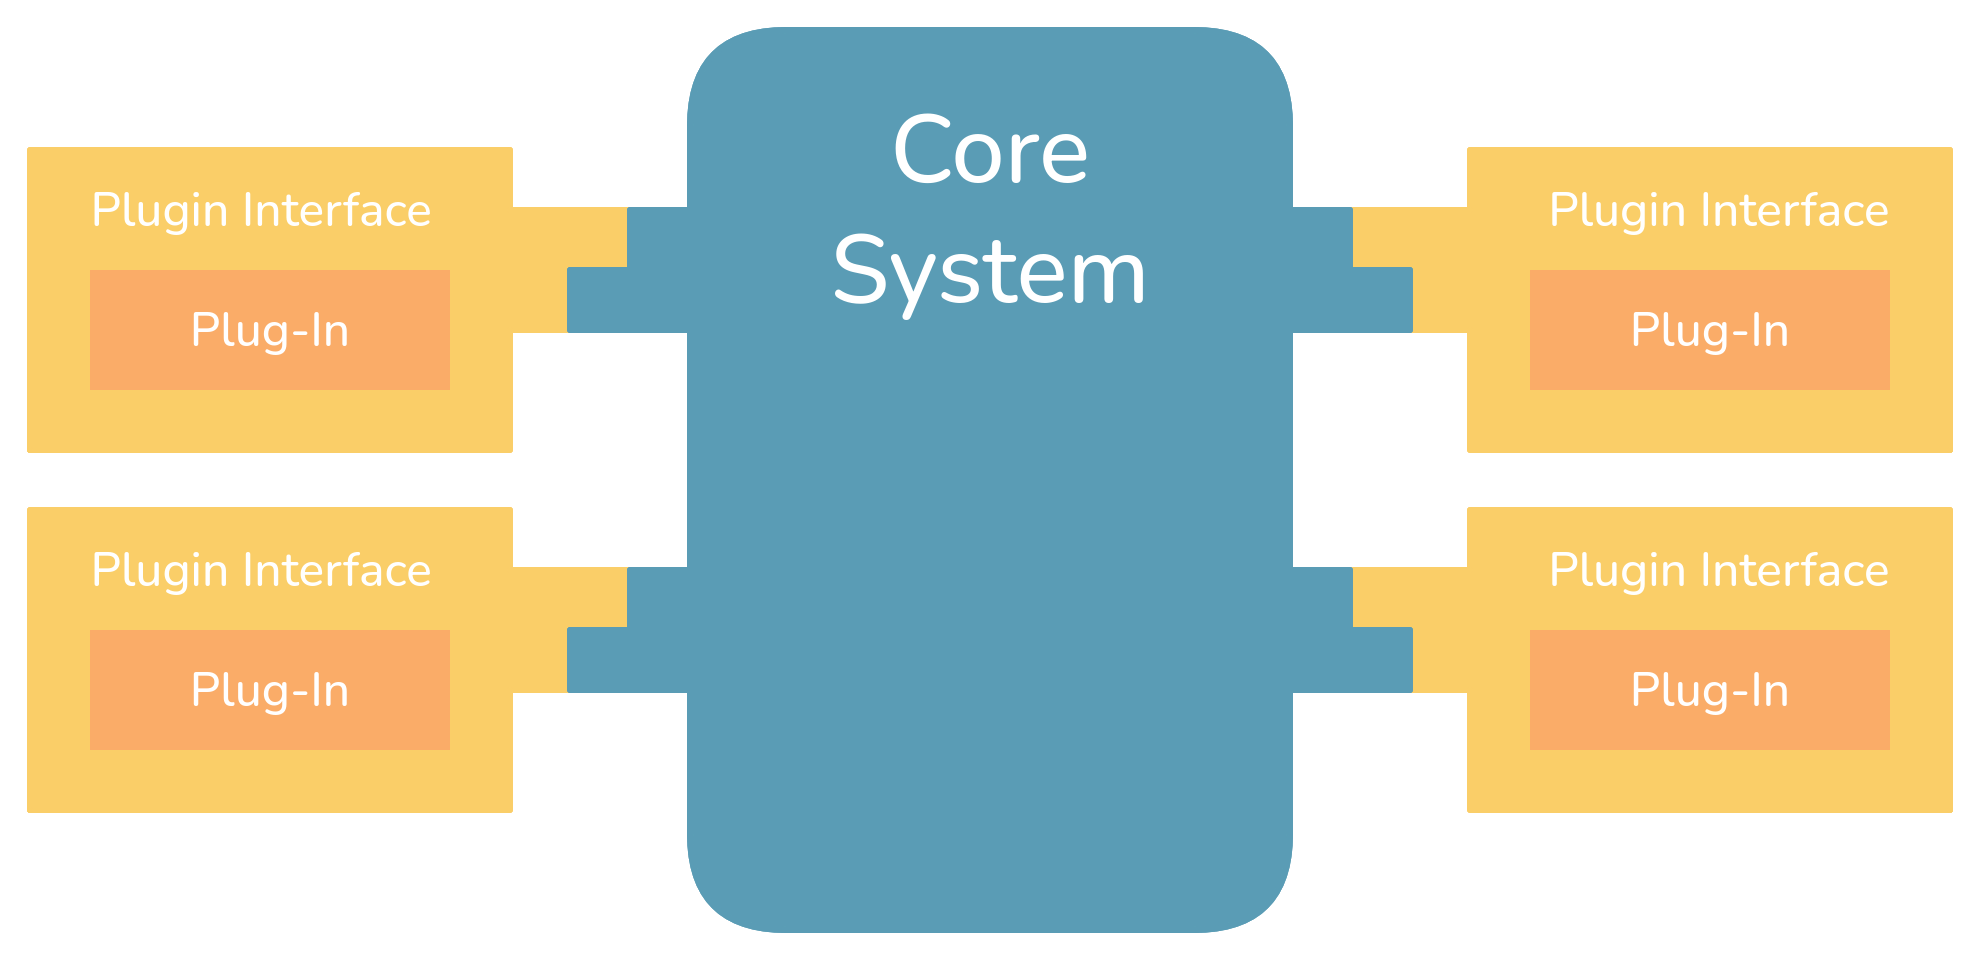
\includegraphics[width=0.6\textwidth]{figures/prelim/PluginDiagram.png}
	\caption{Illustration of a plugin architecture, where independently developed plugins extend a core system through a defined plugin interface.}
	\label{fig:plugin_architecture}
\end{figure}

The plugin architecture is a well-established and widely used approach for building extensible software systems~\cite{plugin-microservice}. As discussed in \cref{chap:related_work}, both KNIME and ProM employ this pattern to support a broad range of extensions, and ProM is an example of a pure plugin system.

\subsection{Microservice Architecture}

While a plugin architecture extends a system by adding components to a shared core, a microservice architecture focuses on decomposing a larger system into smaller, independently deployable services.
In this approach, an application is structured as a collection of small, independent services.
Each service is responsible for a specific business capability and manages its own data, logic, and deployment lifecycle.
Communication between services typically occurs through lightweight mechanisms such as REST interfaces or message queues.

\begin{figure}[htbp]
	\centering
	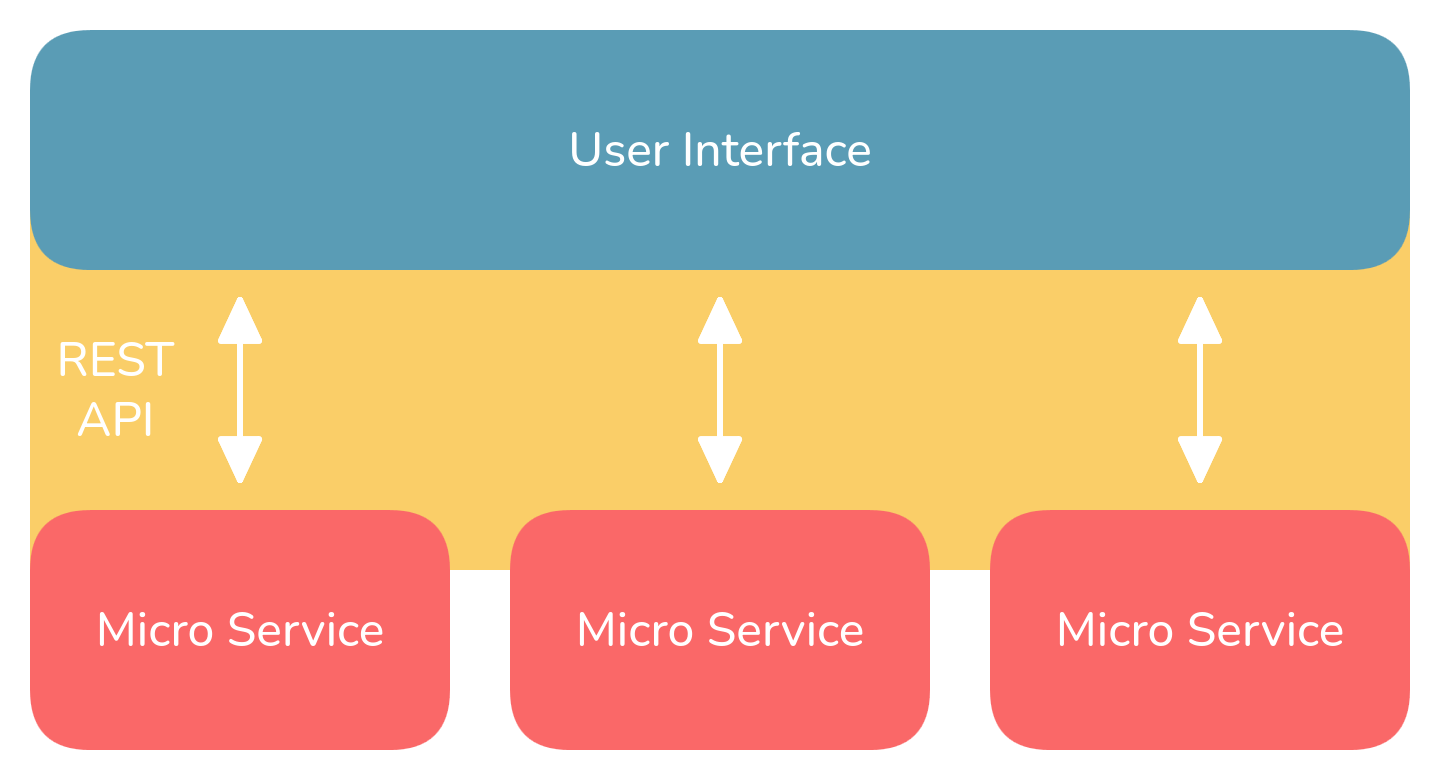
\includegraphics[width=0.6\textwidth]{figures/prelim/MicroService.png}
	\caption{Illustration of a microservice architecture, where independent services communicate with a user interface through a REST API.}
	\label{fig:microservice_architecture}
\end{figure}

The main advantages of this architecture include independent scalability and flexibility in how services are built and deployed.
Microservices are widely used in distributed and cloud-native systems, where individual services can be deployed, updated, and scaled separately~\cite{plugin-microservice}.

\subsection{Microfrontend Architecture}

A microfrontend architecture applies the principles of microservices to the frontend. Instead of implementing a single monolithic user interface, the application is composed of multiple smaller frontend units that are developed and deployed independently. These units are integrated at runtime to create a cohesive user experience~\cite{plugin-microservice}.

\begin{figure}[htbp]
	\centering
	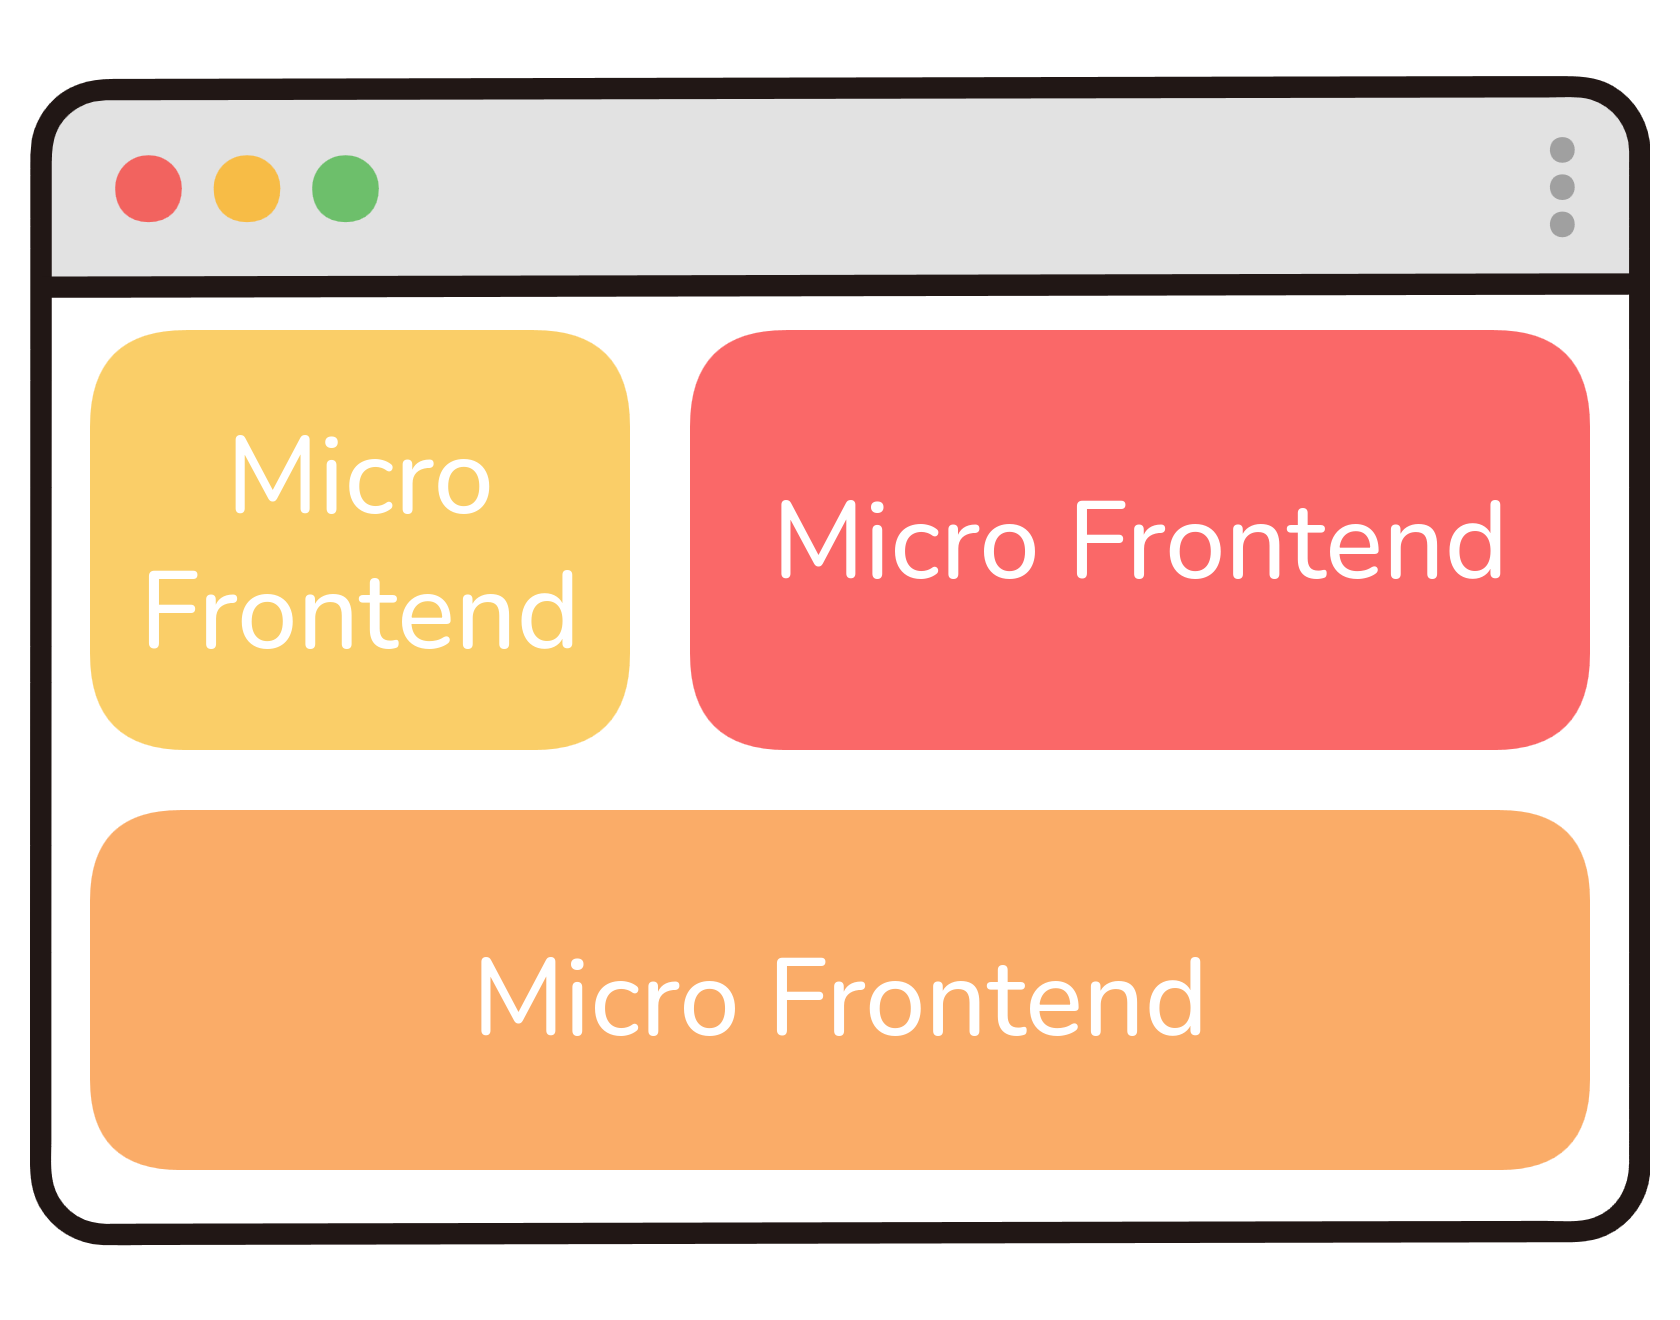
\includegraphics[width=0.5\textwidth]{figures/prelim/MicroFrontend.png}
	\caption{Illustration of a microfrontend architecture, where multiple independently developed frontend components are combined into a single user interface.}
	\label{fig:microfrontend_architecture}
\end{figure}

This approach allows teams to work on different parts of the interface independently. A practical example is Celonis Views, where dashboards are created by combining multiple view components into a single application.

\section{Software Development Techniques}

In addition to architectural patterns, these software engineering practices were essential for the development of Ocelescope.

\subsection{JSON and JSON Schema}

JSON (JavaScript Object Notation) is a text-based format for exchanging data and is widely used on the web. A JSON document is a collection of key--value pairs. Values can be strings, numbers, booleans, arrays, or nested JSON objects.
This simple structure makes JSON efficient for machines to process and straightforward for humans to read.
Common use cases include representing data in HTTP request and response bodies and storing documents in NoSQL databases~\cite{json}.
JSON is also one of the exchange formats supported by the \textit{OCEL~2.0} standard~\cite{ocel2}.


JSON Schema is a language for specifying the structure of JSON documents. A JSON Schema is itself written in JSON. It explains which properties may appear in a document, which properties must be present, and what type each value should have. It can also express more complex structures. For example, it can describe values that may follow one of several allowed types or define rules for arrays and nested objects. In addition, it can limit numbers to a certain range or require that strings follow a specific pattern. JSON Schema is widely used in OpenAPI to describe and validate the inputs and outputs of RESTful APIs~\cite{json}.

\subsection{Containerization}

Containerization is a lightweight form of virtualization. It allows applications to run in isolated environments while still being tightly integrated with the host operating system. Containers are small in size, have fast startup times, can communicate with each other, can mount directories from the host system, and provide near-native performance~\cite{docker}.

Docker is a widely used tool for managing containers. Containers are created from build scripts, and the resulting images are binary artifacts that can be executed directly or uploaded to a container registry. These images can be run on Linux, macOS, and Windows. Docker also supports communication between containers and is widely used in the deployment of cloud services~\cite{dockerinscience}. It is also commonly used in microservice architectures, where each service is deployed in its own container.
